% Foliensatz: "AFu-Kurs nach DJ4UF" von DK0TU, Amateurfunkgruppe der TU Berlin
% Lizenz: CC BY-NC-SA 3.0 de (http://creativecommons.org/licenses/by-nc-sa/3.0/de/)
% Autoren: Martin Deutschmann, Lars Weiler <dc4lw@darc.de>

preamble.dk0tu.tex
\subtitle{Technik Klasse E 05: \\
          Der Kondensator und seine Schaltungsarten \\[2em]}
\date{Stand 26.10.2015}
 \begin{document}

\begin{frame}
    \titlepage
    \vfill
    \begin{center}
        \ccbyncsaeu\\
        {\tiny This work is licensed under the \em{Creative Commons Attribution-NonCommercial-ShareAlike 3.0 License}.}\\[0.5ex]
         \tiny Amateurfunkgruppe der Technische Universität Berlin (AfuTUB), DKØTU
         %\includegraphics[scale=0.5]{img/DK0TU_Logo.pdf}
    \end{center}
\end{frame}


\section*{Einleitung}

\begin{frame}
    \frametitle{Einleitung / Kondensator}
    \begin{center}
        \Large{Wie sieht er aus?}\\
        \Large{Was tut der?}         
    \end{center}
\end{frame}


\begin{frame}
    \frametitle{Einleitung / Kondensator}

    \begin{center}
        \includegraphics[width=0.7\textwidth]{e05/Kondensator01.jpg}
        \footnote{Abb.1: Verschiedene Kondensatoren \cite{wmen}}
    \end{center}
 	

\end{frame}

\begin{frame}
    \frametitle{Einleitung / Kondensator}

    \begin{center}
        \includegraphics[width=0.8\textwidth]{e05/Kondensator02.jpg}
        \footnote{Abb.2: Verschiedene kleine Kondensatoren \cite{wmen}}
    \end{center}
\end{frame}

\section*{Anwendungen}
\begin{frame}
  \frametitle{Diverse Anwendungsmöglichkeiten}
  \only<1>{Bisher kam ich ganz gut ohne Kondensatoren im Leben aus\ldots}
  \pause
  \begin{itemize}
    \item Energiespeicher
    \item Blitzlicht 
    \item Signalentkopplung
    \item Filter 
    \item Schwingkreise 
    \item Glättung 
    \item Entstörung 
    \item Phasenkompensation 
  \end{itemize}
\end{frame}


\section*{Kapazität}

\begin{frame}
    \frametitle{Kapazität}
	
	\begin{center}
        \includegraphics[width=0.8\textwidth]{e05/c-aufbau.png}
        \footnote{Abb.3: Interner Aufbau eines Plattenkondensators \cite{wp}}
    \end{center}
\end{frame}

\section*{Gleich\-strom\-kreis}
\begin{frame}
	\frametitle{ein paar Formeln}
	\begin{block}{Berechnung eines Kondensators}
	  \begin{center}
	    \huge{$C = \frac{Q}{U}$} in $[C] = \frac{As}{V} = F$ (Farad)
	  \end{center}
	  Ladung des Kondensators im Verhältnis zur Spannung
	\end{block}
	\begin{block}{Berechnung eines Kondensators}
	  \begin{center}
	    \huge{$C= \varepsilon_{0} \cdot \varepsilon_{r} \cdot \cfrac{A}{d}$}\\
	      \small{mit $\varepsilon_{0} = 0,885 \cdot 10^{-11} \frac{As}{Vm}$: Elektrische Feldkonstante\\
	      $\varepsilon_{r}$: relative Dielektrizitätszahl}
	  \end{center}
	\end{block}
	Sobald der Kondensator geladen ist, fließt kein Strom mehr.
\end{frame}

\section{Wechsel\-strom\-kreis}
\begin{frame}
  \frametitle{Funktionsprinzip im Wechselstromkreis}
  \begin{columns}
    \column{0.37\textwidth}
      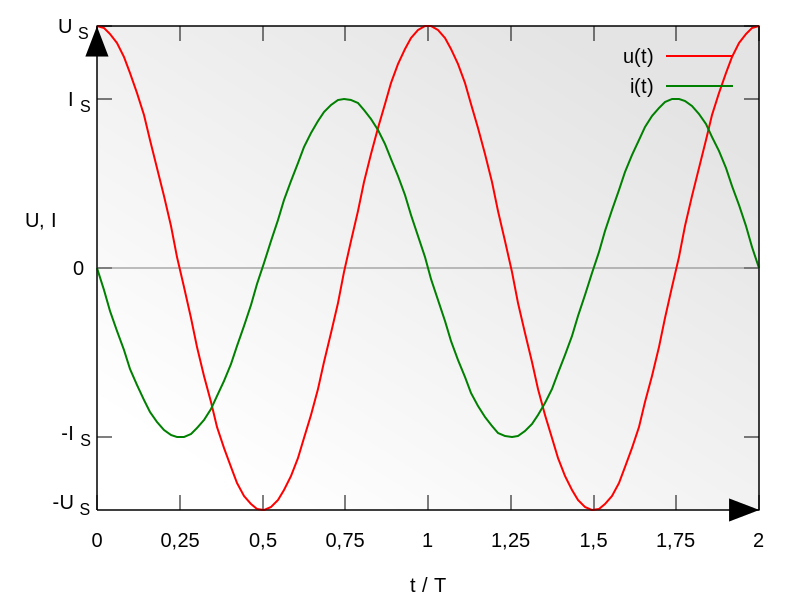
\includegraphics[width=1\textwidth]{e05/Sinus_Voltage_and_Current_of_a_Capacitor.png}\footnotemark
    \column{0.63\textwidth}
    {\small
    \begin{block}{}
    \begin{description}
      \item[$t=0$] Kondensator ist geladen; es fließt kein Strom
      \item[$0<t<0,25$] Kondensator wird entladen; der Stromfluss nimmt zu
      \item[$t=0,25$] Kondensator ist entladen; der Stromfluss ist am Maximum 
      \item[$0,25<t<0,5$] Kondensator wird umgekehrt aufgeladen; der Stromfluss in diese Richtung nimmt ab
      \item[$t=0,5$] Kondensator ist umgekehrt aufgeladen; es fließt kein Strom
    \end{description}
    \end{block}
    }
  \end{columns}
  \footnotetext[4]{\tiny Abb.: CC-BY-SA 3.0 Fabian R \url{https://de.wikipedia.org/wiki/Datei:Sinus_Voltage_and_Current_of_a_Capacitor.svg}}
\end{frame}

\begin{frame}
    \frametitle{Eselsbrücke}
  \begin{block}{Merksatz}
    Kondensator: Strom eilt vor
  \end{block}
\end{frame}

\begin{frame}
  \frametitle{Kapazitiver Widerstand}

  Abhängig von der Frequenz $f$.

  \begin{block}{Impedanz als Scheinwiderstand}
    \huge{$X_C = \frac{1}{2 \cdot \pi \cdot f \cdot C}$}
  \end{block}

  \pause
  Der Scheinwiderstand sinkt bei zunehmender Frequenz.\\
  Der Scheinwiderstand sinkt bei größerer Kapazität.
\end{frame}

\begin{frame}
  \begin{center}
      \begin{tabular}{|l|l|p{1cm}|}
	\hline
		\multicolumn{3}{|c|}{\textbf{TC208: Mit zunehmender Frequenz...}}\\
		\hline
		A & steigt der Wechselstromwiderstand des Kondensators. & ??? \\ \hline
		B & sinkt der Wechselstromwiderstand des Kondensators. & \only<1>{???}\only<2>{richtig} \\ \hline
		C & steigt der Wechselstromwiderstand des Kondensators  & ??? \\
		" " & bis zu einem Maximum und sinkt dann wieder. & " " \\ \hline
		D & sinkt der Wechselstromwiderstand des Kondensators & ??? \\
		" " & bis zu einem Minimum und steigt dann wieder. & " " \\ \hline
	\end{tabular}
  \end{center}
\end{frame}


\section*{Schaltungsarten}

\subsection*{Parallel\-schaltung}

\begin{frame}
    \frametitle{Parallelschaltung von Kondensatoren}
    \begin{center}
        \includegraphics[width=0.7\textwidth]{e05/c-parallel.png}
        \footnote{\tiny By Martin Deutschmann mit Eagle}
    \end{center}
    \begin{block}{Parallelschaltung}
      $C_{ges} = C_1 + C_2 + C_3 + C_4 + C_5$
    \end{block}
\end{frame}
	
\begin{frame}
  \begin{exampleblock}{TC206}
    Drei Kondensatoren mit den Kapazitäten $C_{1} = 0,1 \mu F, C_{2} = 150 nF$ und $C_{3} = 50000 pF$ werden parallel geschaltet. Wie groß ist die Gesamtkapazität?
  \end{exampleblock}
  \pause
  \begin{center}
    $C_{ges} = C_1 + C_2 + C_3 = 0,1 \mu F + 150 nF + 50000 pF = 0,3 \mu F$
  \end{center}
\end{frame}

\subsection*{Reihen\-schaltung}

\begin{frame}
  \frametitle{Reihenschaltung von Kondensatoren}
  \begin{center}
    \includegraphics[width=0.6\textwidth]{e05/c-reihe.png}\footnote{\tiny By Martin Deutschmann mit Eagle}
  \end{center}
  \begin{block}{Reihenschaltung}
      $\frac{1}{C_{ges}} = \frac{1}{C_1} + \frac{1}{C_2} + \frac{1}{C_3} + \frac{1}{C_4} + \frac{1}{C_5}$\\
      $C_{ges} = \cfrac{1}{\frac{1}{C_1} + \frac{1}{C_2} + \frac{1}{C_3} + \frac{1}{C_4} + \frac{1}{C_5}}$
  \end{block}
\end{frame}
 
\begin{frame}
  \begin{exampleblock}{Reihenschaltung}
    Zwei Kondensatoren von $100 pF$ und $150 pF$ sind hintereinander (in Serie) geschaltet. Berechnen Sie die Gesamtkapazität.
  \end{exampleblock}
  \pause
  \begin{center}
    $C_{ges} = C_1 \parallel C_2 = 100 pF \parallel 150 pF = \cfrac{1}{\frac{1}{100 pF} + \frac{1}{150 pF}} = 60 pF$
  \end{center}
\end{frame}

\begin{frame}
  \begin{alertblock}{Hausaufgabe}
    Aus Fragenkatalog Klasse E Fragen TB610--TB613.\\
    Aus Fragenkatalog Klasse E Kapitel 1.3.2 Kondensator (Fragen TC201--TC208).
  \end{alertblock}
\end{frame}



\renewcommand{\refname}{Referenzen}

\hypertarget{refs}{}
\textcolor{white}{} \\ %\vspace{} geht nicht
\Large Referenzen/Links
\footnotesize

\begin{thebibliography}{}
    \bibitem{e03}   Moltrecht E 05: \\
                    \url{http://www.darc.de/referate/ajw/ausbildung/darc-online-lehrgang/technik-klasse-e/technik-e05/}
    \bibitem{wp}    Wikipedia DE: \\
                    \url{http://de.wikipedia.org/wiki/Kondensator_(Elektrotechnik)}\\ 
    \bibitem{wmde}	Wikimedia DE:\\
    				\url{http://de.wikipedia.org/wiki/Datei:Plate_Capacitor_DE.svg}\\
   	\bibitem{wmen}	Wikimedia EN:\\
   					\url{http://commons.wikimedia.org/wiki/File:Capacitors_(7189597135).jpg}\\
   					\url{http://commons.wikimedia.org/wiki/File:Condensators.JPG}
\end{thebibliography} 

% Hier könnte noch eine Kontaktfolie stehen

\end{document}

